\documentclass[a4paper]{article}

\usepackage[pages=all, color=black, position={current page.south}, placement=bottom, scale=1, opacity=1, vshift=5mm]{background}
%\SetBgContents{
%	\tt This work is shared under a \href{https://creativecommons.org/licenses/by-sa/4.0/}{CC BY-SA 4.0 license} unless otherwise noted
%}      % copyright

\usepackage[margin=1in]{geometry} % full-width

% AMS Packages
\usepackage{amsmath}
\usepackage{amsthm}
\usepackage{amssymb}

% Unicode
\usepackage[utf8]{inputenc}
\usepackage{hyperref}
\hypersetup{
	unicode,
%	colorlinks,
%	breaklinks,
%	urlcolor=cyan, 
%	linkcolor=blue, 
	pdfauthor={Author One, Author Two, Author Three},
	pdftitle={A simple article template},
	pdfsubject={A simple article template},
	pdfkeywords={article, template, simple},
	pdfproducer={LaTeX},
	pdfcreator={pdflatex}
}

% Vietnamese
%\usepackage{vntex}

% Natbib
\usepackage[sort&compress,numbers,square]{natbib}
\bibliographystyle{mplainnat}

% Theorem, Lemma, etc
\theoremstyle{plain}
\newtheorem{theorem}{Theorem}
\newtheorem{corollary}[theorem]{Corollary}
\newtheorem{lemma}[theorem]{Lemma}
\newtheorem{claim}{Claim}[theorem]
\newtheorem{axiom}[theorem]{Axiom}
\newtheorem{conjecture}[theorem]{Conjecture}
\newtheorem{fact}[theorem]{Fact}
\newtheorem{hypothesis}[theorem]{Hypothesis}
\newtheorem{assumption}[theorem]{Assumption}
\newtheorem{proposition}[theorem]{Proposition}
\newtheorem{criterion}[theorem]{Criterion}
\theoremstyle{definition}
\newtheorem{definition}[theorem]{Definition}
\newtheorem{example}[theorem]{Example}
\newtheorem{remark}[theorem]{Remark}
\newtheorem{problem}[theorem]{Problem}
\newtheorem{principle}[theorem]{Principle}

\usepackage{graphicx, color}
\graphicspath{{fig/}}

%\usepackage[linesnumbered,ruled,vlined,commentsnumbered]{algorithm2e} % use algorithm2e for typesetting algorithms
\usepackage{algorithm, algpseudocode} % use algorithm and algorithmicx for typesetting algorithms
\usepackage{mathrsfs} % for \mathscr command

%\usepackage{lipsum}

% Author info
\title{Andy's science scratch pad}
\author{J. Andrew Fingerhut$^1$}

\date{
	$^1$\texttt{andy.fingerhut@gmail.com}
%	\today
}

\newcommand{\ihat}{\textbf{i}}
\newcommand{\jhat}{\textbf{j}}
\newcommand{\khat}{\textbf{k}}
\newcommand{\rhat}{\hat{\textbf{r}}}
\newcommand{\vect}[1]{\textbf{#1}}

\begin{document}
\maketitle

\begin{abstract}
  todo: abstract here
\end{abstract}

\tableofcontents

\section{Introduction}
\label{sec:intro}

This document is a place to write up little bits on science.

Some notation:

$\ihat$ is the unit vector from left to right.
$\jhat$ is the unit vector upwards.
$\khat$ is the unit vector pointed out of the page toward the reader.

$\gamma = 1/\sqrt{1-v^2/c^2}$ is the Lorentz factor.


\section{Electromagnetic force between two point charges at rest relative to each other}
\label{sec:twocharges}

%Now we include a figure.
%(See Figure~\ref{fig:example}.)
%\begin{figure}[ht]
%	\centering
%	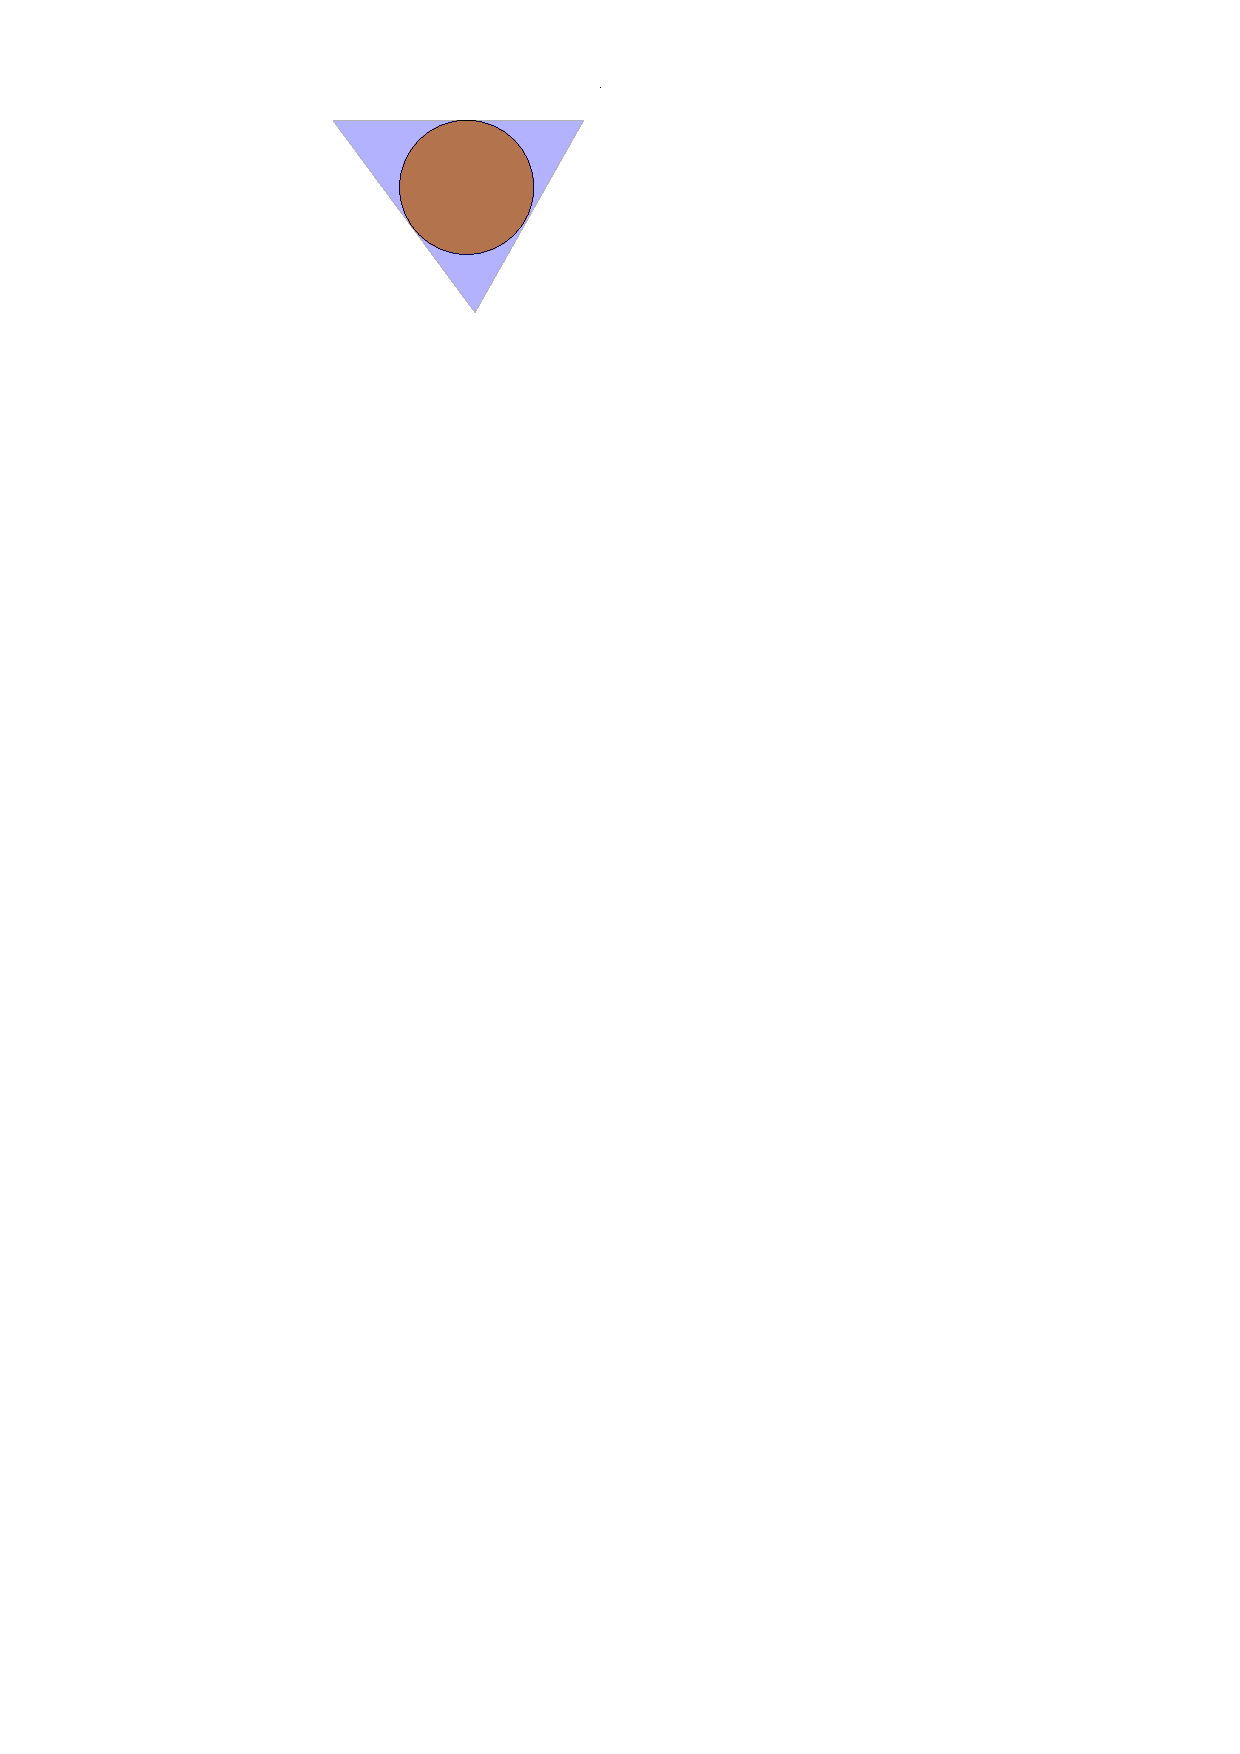
\includegraphics[width=0.3\textwidth]{example}
%	\caption{An example of a figure}
%	\label{fig:example}
%\end{figure}

Scenario 1: There are two point charges $a$ and $b$ both with charge
$q$ at rest relative to each other at a distance $r$ apart (in the
horizontal, i.e. left-right direction, on this page).  They are at
rest relative to us.  In this case they both experience a force
directly away from the other due to electric repulsion.  There is no
magnetic force, as both charges are at rest so there are no magnetic
fields.


Scenario 2: The same as scenario 1, but both charges are moving with
constant velocity $v$ in the upwards direction.  Thus they are at rest
relative to each other, as they are in scenario 1.

Each charge creates an electric field, but since they are moving they
also create magnetic fields.

Questions:
\begin{itemize}
  \item What is the net force on charge $b$ in each scenario?
  \item Is it the same in both scenarios, or different?
  \item Why?
\end{itemize}


\subsection{Scenario 1: Both charges at rest}

As mentioned before, there is no current or motion of any charges in
this scenario, so no magnetic fields.  The electric repulsion force on
charge $b$ is easily calculated from Coulomb's Law~\cite{CoulombsLaw}.
Charge $b$ is to the right of charge $a$, so the direction of the force is
$\ihat$, away from charge $a$.

\begin{equation}
\vect{E}_1 = \frac{1}{4 \pi \epsilon_0} \frac{q}{r^2} \ihat \label{eq:E1}
\end{equation}

\begin{equation}
\vect{B}_1 = 0
\end{equation}

\begin{equation}
\vect{F}_1 = q(\vect{E}_1 + \vect{v} \times \vect{B}_1)
           = q \vect{E}_1   \label{eq:F1}
\end{equation}


\subsection{Scenario 2: Both charges with equal and constant velocity upwards}

The Wikipedia page on the Biot-Savart
Law~\cite{EMFieldFromPointCharge} has a subsection titled ``Point
charge at constant velocity'' that says:

\begin{quote}
the Biot–Savart law applies only to steady currents and a point charge
moving in space does not constitute a steady current
\end{quote}

I will thus use the equations in that section to calculate the
electric and magnetic fields here.  The relevant parts of the
Wikipedia page are copied below.

\begin{quote}
In the case of a point charged particle $q$ moving at a constant
veclocity $v$, Maxwell's equations give the following expression for
the electric field and magnetic field:
\end{quote}
\begin{align}
\vect{E} & = \frac{q}{4 \pi \epsilon_0} \frac{1-\beta^2}{(1-\beta^2 \sin^2 \theta)^{3/2}} \frac{{\rhat}'}{|r'|^2} \label{eq:EforPtChg} \\
\vect{B} & = \frac{1}{c^2} \vect{v} \times \vect{E} \label{eq:BforPtChg}
\end{align}
where:
\begin{itemize}
    \item ${\rhat}'$ is the unit vector pointing from the current
      (non-retarded) position of the particle to the point at which
      the field is being measured,
    \item $\beta = v/c$ is the speed in units of $c$, and
    \item $\theta$ is the angle between $\vect{v}$ and ${\rhat}'$.
      Alternatively, these can be derived by considering the Lorentz
      tranfromation of the Coulomb's force (in four-force form) in the
      source charge's inertial frame.
\end{itemize}

Calculation: To get the force on charge $b$, we first calculate the
$\vect{E}$ and $\vect{B}$ fields at the position of charge $b$.

Charge $b$ is directly to the right of charge $a$, so ${\rhat}' = \ihat$
and $\theta = 90^{\circ}$.

\begin{align}
\vect{E}_2
  & = \frac{q}{4 \pi \epsilon_0} \frac{1-\beta^2}{(1-\beta^2 \sin^2 \theta)^{3/2}} \frac{{\rhat}'}{|r'|^2} & & \text{${\rhat}' = \ihat$, $|r'| = r$, $\theta=90^{\circ}$, simplify fraction} \nonumber \\
  & = \frac{q}{4 \pi \epsilon_0} \frac{1}{(1-\beta^2)^{1/2}} \frac{\ihat}{r^2} & & \text{part of this is $\gamma$, by~\eqref{eq:E1} the rest is $\vect{E}_1$} \nonumber \\
  & = \gamma \vect{E}_1 \label{eq:E2value}
\end{align}

\begin{align*}
\vect{F}_2
  & = q (\vect{E}_2 + \vect{v} \times \vect{B}_2)   & & \text{replace $\vect{B}_2$ with \eqref{eq:BforPtChg}} \\
  & = q (\vect{E}_2 + \vect{v} \times (\frac{1}{c^2} \vect{v} \times \vect{E}_2))  & & \vect{v} \times \vect{E}_2 = - v E_2 \khat \\
  & = q (\vect{E}_2 - \frac{v E_2}{c^2} \vect{v} \times \khat)  & & \vect{v} \times \khat = v \ihat \\
  & = q (\vect{E}_2 - \frac{v^2 E_2}{c^2} \ihat) \\
  & = q (1 - \frac{v^2}{c^2}) \vect{E}_2 \\
  & = \frac{q \vect{E}_2}{\gamma^2} & & \text{by~\eqref{eq:E2value} \ } \vect{E}_2 = \gamma \vect{E}_1 \\
  & = \frac{q \vect{E}_1}{\gamma} & & \text{by~\eqref{eq:F1} \ } \vect{F}_1 = q \vect{E}_1 \\
  & = \frac{\vect{F}_1}{\gamma}
\end{align*}

Thus $\vect{F}_2$ differs from $\vect{F}_1$ by a factor of $\gamma$.

TODO: Why?

I do not know how to check the answer below, but it appears that three
of the answers to an on-line question similar to
mine~\cite{PhysicsSEIsLorentzForceFrameIndependent} say that the
Lorentz force formula $\vect{F} = q(\vect{E} + \vect{v} \times
\vect{B})$ is {\em not} invariant in all inertial frames, but perhaps
a variant of it is.  I quote one such answer below:

\begin{quote}
Just for completeness if permitted: Following Section 3.1 from the
book ``Gravitation'' of Misner, Thorne, and Wheeler the truly (at all
speeds) frame independent force is $\frac{dP}{d \tau} = \gamma (E + v
\times B)$ (in fact this is only the spacial component of the four
force).  $\tau$ is proper time and $\gamma$ the well-known Lorentz
Factor. -- Kurt G. Aug 28, 2021
\end{quote}


%\newpage
\bibliography{refs}

%\appendix

%\section{Omitted Proof in Section~\ref{sec:examples}}
%\label{app:1}

	
\end{document}
